
\documentclass[dvipdfmx]{standalone}
\usepackage[T1]{fontenc}
\usepackage{newtxtext, newtxmath}

\usepackage{tikz}
\usetikzlibrary{positioning}
% \usetikzlibrary{fit}
% calc, positioning, quotes, topaths, scopes, spy
% matrix, graphs, graph.standard, trees, chains, automata, mindmap, er, calendar
% shapes.(geometric|symbols|arrows|multipart|callouts|misc)?
% arrows, patterns, fadings, shadings, shadows, backgrounds
% circuits.logic.US, circuits.ee.IEC, lindenmayersystems, folding, petri, svg.path
% decorations.(pathmorphing|pathreplacing|markings|footprints|shapes|text|fractals)?
% datavisualization, datavisualization.formats.functions
% intersections, plothandlers, plotmarks, through

\begin{document}
  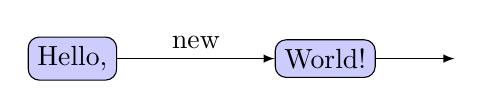
\begin{tikzpicture}[> = latex]
    \tikzset{
      int/.style={draw, fill=blue!20, rounded corners},
    }
    \node [int] (a) {Hello,};
    \node [int, right=2cm of a] (b) {World!};
    \coordinate [right=1cm of b] (c);
    \path[->] (a) edge node[above] {new} (b) (b) edge (c);

  \end{tikzpicture}
\end{document}
